\documentclass[a4paper,12pt]{scrartcl}

\usepackage{/home/patrick/LaTeX/mesmacros/exercice_sheet}

%\trait
%\section*{}
%\exo{}
%\question{}
%\subquestion{}

\date{}


% Title Page
\title{Dérivation}

\author{\textsc{Mathématiques}}

\begin{document}

\selectlanguage{french}

\maketitle

\tableofcontents

\section*{Introduction}

La dérivée d'une fonction est une notion fondamentale en mathématiques et présente une multitude d'applications. 

Elle indique les variations de la grandeur étudiée.

Par exemple si la variable $t$ est le temps et que $f$ est la fonction indiquant la position d'un objet à tout instant $t$, $f(t)$ est la position de l'objet à cet instant $t$. Alors $f'(t)$, la dérivée de la fonction $f$ représente la vitesse de l'objet à l'instant $t$. 

Mais ce n'est pas tout, la dérivée de la dérivée ($f''(t)$) représente l'accélération de l'objet.

De façon plus générale, la dérivée exprime la variation d'une grandeur (ici représentée par une fonction).

De façon plus précise, soit une fonction $f:x \longmapsto f(x)$. La dérivée compare la variation de $x$ à la variation de $f(x)$ correspondante. D'où la notation $\dfrac{\ud{} f(x)}{\ud{} x}$ où $\ud{}$ sert à exprimer une variation infinitésimale de l'élément qui le suit.

\part{Le nombre dérivé} 

\section{Rappel: équation d'une droite} 

L'équation d'une droite $(D)$ non parallèle à l'axe des ordonnées est de la forme: $y = ax+b$ où $a$ et $b$ sont des nombres réels.

\begin{enumerate}
 \item $a$ est appelé le \emph{coefficient directeur}; 
 \item $b$ est appelé l'\emph{ordonnée à l'origine}. C'est l'ordonnée du point d'intersection de la droite $(D)$ avec l'axe des ordonnées $(Oy)$.
\end{enumerate}

Pour deux points $M_1(x_1;y_1)$ et $M_2(x_2;y_2)$ appartenant à cette droite nous avons:

\begin{equation*}
 a = \frac{\Delta y}{\Delta x} = \frac{y_1 - y_2}{x_1 - x_2}
\end{equation*}

\begin{center}
\input{pics/droite.txt}
\end{center}

\exemple{Déterminer le coefficient directeur $a$ et l'ordonnée à l'origine $b$ de la droite $(D)$ tracée dans le repère ci-dessous.}

\begin{center}
  \simpleplot{-1}{3}{\x}{4-2*\x}{$(D)$}{1}
\end{center}

\cadre{4}


\section{Tangente à la courbe représentative d'une fonction et nombre dérivé.}  

\subsection{La tangente}

Soit une fonction $f$ dont la représentation graphique est une courbe $\mathcal{C}_f$ d'équation $y  = f(x)$.
On considère sur $\mathcal{C}_f$ un point fixe $M_0$ d'abscisse $x_0$ et d'ordonnée $y_0 = f(x_0)$:  $M_0(x_0 ; f(x_0))$ et un point M non fixe appartenant à $\mathcal{C}_f$.

Si on fait tendre $M$ vers le point $M_0$ ($M$ se rapproche de plus en plus près de $M_0$) la droite $(M_0M)$ tend vers une droite limite qui est la tangente $\mathcal{T}$ à la courbe $\mathcal{C}$ au point $M_0$.

\begin{center}
% \documentclass[10pt]{article}
% \usepackage{pgf,tikz,pgfplots}
% \pgfplotsset{compat=1.15}
% \usepackage{mathrsfs}
% \usetikzlibrary{arrows}
% \pagestyle{empty}
% \begin{document}
\definecolor{ududff}{rgb}{0.30196078431372547,0.30196078431372547,1}
\definecolor{qqqqyq}{rgb}{0,0,0.5019607843137255}
\definecolor{yqyqyq}{rgb}{0.5019607843137255,0.5019607843137255,0.5019607843137255}
\definecolor{xdxdff}{rgb}{0.49019607843137253,0.49019607843137253,1}
\definecolor{qqwuqq}{rgb}{0,0.39215686274509803,0}
\begin{tikzpicture}[line cap=round,line join=round,>=triangle 45,x=1cm,y=1cm]
\begin{axis}[
% %x=1cm,y=1cm,
axis lines=middle,
scale=2,
ymajorgrids=true,
xmajorgrids=true,
yminorgrids=true,
xminorgrids=true,
xmin=-0.6264641968689706,
xmax=3.4040458021198274,
ymin=-0.38991695131949167,
ymax=3.025894262435394,
xtick={-0.6000000000000001,-0.4000000000000001,...,3.4},
ytick={-0.2,0,...,3},]
\clip(-0.6264641968689706,-0.38991695131949167) rectangle (3.4040458021198274,3.025894262435394);
\draw[line width=1pt,color=qqwuqq] (-0.6264641968689706,0.27542145564135834) -- (-0.6264641968689706,0.27542145564135834);
\draw[line width=1pt,color=qqwuqq] (-0.6264641968689706,0.27542145564135834) -- (-0.6163879218714986,0.2886285605712352);
\draw[line width=1pt,color=qqwuqq] (-0.6163879218714986,0.2886285605712352) -- (-0.6063116468740266,0.3017848998421998);
\draw[line width=1pt,color=qqwuqq] (-0.6063116468740266,0.3017848998421998) -- (-0.5962353718765546,0.31489047345425203);
\draw[line width=1pt,color=qqwuqq] (-0.5962353718765546,0.31489047345425203) -- (-0.5861590968790826,0.327945281407392);
\draw[line width=1pt,color=qqwuqq] (-0.5861590968790826,0.327945281407392) -- (-0.5760828218816106,0.34094932370161946);
\draw[line width=1pt,color=qqwuqq] (-0.5760828218816106,0.34094932370161946) -- (-0.5660065468841387,0.35390260033693466);
\draw[line width=1pt,color=qqwuqq] (-0.5660065468841387,0.35390260033693466) -- (-0.5559302718866667,0.3668051113133376);
\draw[line width=1pt,color=qqwuqq] (-0.5559302718866667,0.3668051113133376) -- (-0.5458539968891947,0.37965685663082804);
\draw[line width=1pt,color=qqwuqq] (-0.5458539968891947,0.37965685663082804) -- (-0.5357777218917227,0.3924578362894062);
\draw[line width=1pt,color=qqwuqq] (-0.5357777218917227,0.3924578362894062) -- (-0.5257014468942507,0.40520805028907214);
\draw[line width=1pt,color=qqwuqq] (-0.5257014468942507,0.40520805028907214) -- (-0.5156251718967787,0.4179074986298257);
\draw[line width=1pt,color=qqwuqq] (-0.5156251718967787,0.4179074986298257) -- (-0.5055488968993067,0.43055618131166684);
\draw[line width=1pt,color=qqwuqq] (-0.5055488968993067,0.43055618131166684) -- (-0.4954726219018347,0.4431540983345956);
\draw[line width=1pt,color=qqwuqq] (-0.4954726219018347,0.4431540983345956) -- (-0.48539634690436273,0.45570124969861214);
\draw[line width=1pt,color=qqwuqq] (-0.48539634690436273,0.45570124969861214) -- (-0.47532007190689074,0.4681976354037163);
\draw[line width=1pt,color=qqwuqq] (-0.47532007190689074,0.4681976354037163) -- (-0.46524379690941875,0.48064325544990816);
\draw[line width=1pt,color=qqwuqq] (-0.46524379690941875,0.48064325544990816) -- (-0.45516752191194676,0.49303810983718765);
\draw[line width=1pt,color=qqwuqq] (-0.45516752191194676,0.49303810983718765) -- (-0.44509124691447477,0.5053821985655548);
\draw[line width=1pt,color=qqwuqq] (-0.44509124691447477,0.5053821985655548) -- (-0.4350149719170028,0.5176755216350095);
\draw[line width=1pt,color=qqwuqq] (-0.4350149719170028,0.5176755216350095) -- (-0.4249386969195308,0.529918079045552);
\draw[line width=1pt,color=qqwuqq] (-0.4249386969195308,0.529918079045552) -- (-0.4148624219220588,0.5421098707971821);
\draw[line width=1pt,color=qqwuqq] (-0.4148624219220588,0.5421098707971821) -- (-0.4047861469245868,0.5542508968898999);
\draw[line width=1pt,color=qqwuqq] (-0.4047861469245868,0.5542508968898999) -- (-0.3947098719271148,0.5663411573237054);
\draw[line width=1pt,color=qqwuqq] (-0.3947098719271148,0.5663411573237054) -- (-0.38463359692964283,0.5783806520985985);
\draw[line width=1pt,color=qqwuqq] (-0.38463359692964283,0.5783806520985985) -- (-0.37455732193217084,0.5903693812145792);
\draw[line width=1pt,color=qqwuqq] (-0.37455732193217084,0.5903693812145792) -- (-0.36448104693469885,0.6023073446716476);
\draw[line width=1pt,color=qqwuqq] (-0.36448104693469885,0.6023073446716476) -- (-0.35440477193722686,0.6141945424698037);
\draw[line width=1pt,color=qqwuqq] (-0.35440477193722686,0.6141945424698037) -- (-0.34432849693975487,0.6260309746090474);
\draw[line width=1pt,color=qqwuqq] (-0.34432849693975487,0.6260309746090474) -- (-0.3342522219422829,0.6378166410893789);
\draw[line width=1pt,color=qqwuqq] (-0.3342522219422829,0.6378166410893789) -- (-0.3241759469448109,0.6495515419107979);
\draw[line width=1pt,color=qqwuqq] (-0.3241759469448109,0.6495515419107979) -- (-0.3140996719473389,0.6612356770733046);
\draw[line width=1pt,color=qqwuqq] (-0.3140996719473389,0.6612356770733046) -- (-0.3040233969498669,0.6728690465768989);
\draw[line width=1pt,color=qqwuqq] (-0.3040233969498669,0.6728690465768989) -- (-0.2939471219523949,0.6844516504215811);
\draw[line width=1pt,color=qqwuqq] (-0.2939471219523949,0.6844516504215811) -- (-0.28387084695492293,0.6959834886073508);
\draw[line width=1pt,color=qqwuqq] (-0.28387084695492293,0.6959834886073508) -- (-0.27379457195745094,0.7074645611342081);
\draw[line width=1pt,color=qqwuqq] (-0.27379457195745094,0.7074645611342081) -- (-0.26371829695997895,0.7188948680021532);
\draw[line width=1pt,color=qqwuqq] (-0.26371829695997895,0.7188948680021532) -- (-0.25364202196250696,0.7302744092111858);
\draw[line width=1pt,color=qqwuqq] (-0.25364202196250696,0.7302744092111858) -- (-0.24356574696503497,0.7416031847613062);
\draw[line width=1pt,color=qqwuqq] (-0.24356574696503497,0.7416031847613062) -- (-0.23348947196756298,0.7528811946525142);
\draw[line width=1pt,color=qqwuqq] (-0.23348947196756298,0.7528811946525142) -- (-0.223413196970091,0.7641084388848098);
\draw[line width=1pt,color=qqwuqq] (-0.223413196970091,0.7641084388848098) -- (-0.213336921972619,0.7752849174581932);
\draw[line width=1pt,color=qqwuqq] (-0.213336921972619,0.7752849174581932) -- (-0.203260646975147,0.7864106303726641);
\draw[line width=1pt,color=qqwuqq] (-0.203260646975147,0.7864106303726641) -- (-0.19318437197767502,0.7974855776282228);
\draw[line width=1pt,color=qqwuqq] (-0.19318437197767502,0.7974855776282228) -- (-0.18310809698020303,0.8085097592248691);
\draw[line width=1pt,color=qqwuqq] (-0.18310809698020303,0.8085097592248691) -- (-0.17303182198273104,0.819483175162603);
\draw[line width=1pt,color=qqwuqq] (-0.17303182198273104,0.819483175162603) -- (-0.16295554698525905,0.8304058254414247);
\draw[line width=1pt,color=qqwuqq] (-0.16295554698525905,0.8304058254414247) -- (-0.15287927198778706,0.841277710061334);
\draw[line width=1pt,color=qqwuqq] (-0.15287927198778706,0.841277710061334) -- (-0.14280299699031507,0.8520988290223309);
\draw[line width=1pt,color=qqwuqq] (-0.14280299699031507,0.8520988290223309) -- (-0.13272672199284308,0.8628691823244156);
\draw[line width=1pt,color=qqwuqq] (-0.13272672199284308,0.8628691823244156) -- (-0.12265044699537109,0.8735887699675878);
\draw[line width=1pt,color=qqwuqq] (-0.12265044699537109,0.8735887699675878) -- (-0.1125741719978991,0.8842575919518477);
\draw[line width=1pt,color=qqwuqq] (-0.1125741719978991,0.8842575919518477) -- (-0.10249789700042711,0.8948756482771953);
\draw[line width=1pt,color=qqwuqq] (-0.10249789700042711,0.8948756482771953) -- (-0.09242162200295512,0.9054429389436306);
\draw[line width=1pt,color=qqwuqq] (-0.09242162200295512,0.9054429389436306) -- (-0.08234534700548313,0.9159594639511535);
\draw[line width=1pt,color=qqwuqq] (-0.08234534700548313,0.9159594639511535) -- (-0.07226907200801114,0.9264252232997641);
\draw[line width=1pt,color=qqwuqq] (-0.07226907200801114,0.9264252232997641) -- (-0.06219279701053914,0.9368402169894623);
\draw[line width=1pt,color=qqwuqq] (-0.06219279701053914,0.9368402169894623) -- (-0.05211652201306714,0.9472044450202483);
\draw[line width=1pt,color=qqwuqq] (-0.05211652201306714,0.9472044450202483) -- (-0.042040247015595146,0.9575179073921218);
\draw[line width=1pt,color=qqwuqq] (-0.042040247015595146,0.9575179073921218) -- (-0.03196397201812315,0.967780604105083);
\draw[line width=1pt,color=qqwuqq] (-0.03196397201812315,0.967780604105083) -- (-0.021887697020651152,0.9779925351591319);
\draw[line width=1pt,color=qqwuqq] (-0.021887697020651152,0.9779925351591319) -- (-0.011811422023179157,0.9881537005542684);
\draw[line width=1pt,color=qqwuqq] (-0.011811422023179157,0.9881537005542684) -- (-0.0017351470257071615,0.9982641002904926);
\draw[line width=1pt,color=qqwuqq] (-0.0017351470257071615,0.9982641002904926) -- (0.008341127971764834,1.0083237343678044);
\draw[line width=1pt,color=qqwuqq] (0.008341127971764834,1.0083237343678044) -- (0.01841740296923683,1.018332602786204);
\draw[line width=1pt,color=qqwuqq] (0.01841740296923683,1.018332602786204) -- (0.028493677966708826,1.0282907055456911);
\draw[line width=1pt,color=qqwuqq] (0.028493677966708826,1.0282907055456911) -- (0.03856995296418082,1.038198042646266);
\draw[line width=1pt,color=qqwuqq] (0.03856995296418082,1.038198042646266) -- (0.04864622796165282,1.0480546140879285);
\draw[line width=1pt,color=qqwuqq] (0.04864622796165282,1.0480546140879285) -- (0.05872250295912482,1.0578604198706787);
\draw[line width=1pt,color=qqwuqq] (0.05872250295912482,1.0578604198706787) -- (0.06879877795659681,1.0676154599945165);
\draw[line width=1pt,color=qqwuqq] (0.06879877795659681,1.0676154599945165) -- (0.0788750529540688,1.077319734459442);
\draw[line width=1pt,color=qqwuqq] (0.0788750529540688,1.077319734459442) -- (0.08895132795154079,1.086973243265455);
\draw[line width=1pt,color=qqwuqq] (0.08895132795154079,1.086973243265455) -- (0.09902760294901278,1.096575986412556);
\draw[line width=1pt,color=qqwuqq] (0.09902760294901278,1.096575986412556) -- (0.10910387794648477,1.1061279639007444);
\draw[line width=1pt,color=qqwuqq] (0.10910387794648477,1.1061279639007444) -- (0.11918015294395676,1.1156291757300205);
\draw[line width=1pt,color=qqwuqq] (0.11918015294395676,1.1156291757300205) -- (0.12925642794142875,1.1250796219003842);
\draw[line width=1pt,color=qqwuqq] (0.12925642794142875,1.1250796219003842) -- (0.13933270293890074,1.1344793024118358);
\draw[line width=1pt,color=qqwuqq] (0.13933270293890074,1.1344793024118358) -- (0.14940897793637273,1.1438282172643748);
\draw[line width=1pt,color=qqwuqq] (0.14940897793637273,1.1438282172643748) -- (0.15948525293384472,1.1531263664580016);
\draw[line width=1pt,color=qqwuqq] (0.15948525293384472,1.1531263664580016) -- (0.1695615279313167,1.162373749992716);
\draw[line width=1pt,color=qqwuqq] (0.1695615279313167,1.162373749992716) -- (0.1796378029287887,1.171570367868518);
\draw[line width=1pt,color=qqwuqq] (0.1796378029287887,1.171570367868518) -- (0.1897140779262607,1.1807162200854078);
\draw[line width=1pt,color=qqwuqq] (0.1897140779262607,1.1807162200854078) -- (0.19979035292373268,1.1898113066433853);
\draw[line width=1pt,color=qqwuqq] (0.19979035292373268,1.1898113066433853) -- (0.20986662792120467,1.1988556275424505);
\draw[line width=1pt,color=qqwuqq] (0.20986662792120467,1.1988556275424505) -- (0.21994290291867666,1.207849182782603);
\draw[line width=1pt,color=qqwuqq] (0.21994290291867666,1.207849182782603) -- (0.23001917791614865,1.2167919723638434);
\draw[line width=1pt,color=qqwuqq] (0.23001917791614865,1.2167919723638434) -- (0.24009545291362064,1.2256839962861714);
\draw[line width=1pt,color=qqwuqq] (0.24009545291362064,1.2256839962861714) -- (0.25017172791109266,1.2345252545495873);
\draw[line width=1pt,color=qqwuqq] (0.25017172791109266,1.2345252545495873) -- (0.26024800290856465,1.2433157471540905);
\draw[line width=1pt,color=qqwuqq] (0.26024800290856465,1.2433157471540905) -- (0.27032427790603664,1.2520554740996817);
\draw[line width=1pt,color=qqwuqq] (0.27032427790603664,1.2520554740996817) -- (0.2804005529035086,1.2607444353863602);
\draw[line width=1pt,color=qqwuqq] (0.2804005529035086,1.2607444353863602) -- (0.2904768279009806,1.2693826310141265);
\draw[line width=1pt,color=qqwuqq] (0.2904768279009806,1.2693826310141265) -- (0.3005531028984526,1.2779700609829807);
\draw[line width=1pt,color=qqwuqq] (0.3005531028984526,1.2779700609829807) -- (0.3106293778959246,1.2865067252929223);
\draw[line width=1pt,color=qqwuqq] (0.3106293778959246,1.2865067252929223) -- (0.3207056528933966,1.2949926239439518);
\draw[line width=1pt,color=qqwuqq] (0.3207056528933966,1.2949926239439518) -- (0.3307819278908686,1.3034277569360686);
\draw[line width=1pt,color=qqwuqq] (0.3307819278908686,1.3034277569360686) -- (0.34085820288834057,1.3118121242692733);
\draw[line width=1pt,color=qqwuqq] (0.34085820288834057,1.3118121242692733) -- (0.35093447788581256,1.3201457259435656);
\draw[line width=1pt,color=qqwuqq] (0.35093447788581256,1.3201457259435656) -- (0.36101075288328455,1.3284285619589455);
\draw[line width=1pt,color=qqwuqq] (0.36101075288328455,1.3284285619589455) -- (0.37108702788075654,1.336660632315413);
\draw[line width=1pt,color=qqwuqq] (0.37108702788075654,1.336660632315413) -- (0.3811633028782285,1.3448419370129685);
\draw[line width=1pt,color=qqwuqq] (0.3811633028782285,1.3448419370129685) -- (0.3912395778757005,1.3529724760516113);
\draw[line width=1pt,color=qqwuqq] (0.3912395778757005,1.3529724760516113) -- (0.4013158528731725,1.3610522494313422);
\draw[line width=1pt,color=qqwuqq] (0.4013158528731725,1.3610522494313422) -- (0.4113921278706445,1.3690812571521604);
\draw[line width=1pt,color=qqwuqq] (0.4113921278706445,1.3690812571521604) -- (0.4214684028681165,1.3770594992140661);
\draw[line width=1pt,color=qqwuqq] (0.4214684028681165,1.3770594992140661) -- (0.4315446778655885,1.3849869756170599);
\draw[line width=1pt,color=qqwuqq] (0.4315446778655885,1.3849869756170599) -- (0.44162095286306047,1.392863686361141);
\draw[line width=1pt,color=qqwuqq] (0.44162095286306047,1.392863686361141) -- (0.45169722786053246,1.40068963144631);
\draw[line width=1pt,color=qqwuqq] (0.45169722786053246,1.40068963144631) -- (0.46177350285800445,1.4084648108725666);
\draw[line width=1pt,color=qqwuqq] (0.46177350285800445,1.4084648108725666) -- (0.47184977785547644,1.4161892246399108);
\draw[line width=1pt,color=qqwuqq] (0.47184977785547644,1.4161892246399108) -- (0.48192605285294843,1.4238628727483427);
\draw[line width=1pt,color=qqwuqq] (0.48192605285294843,1.4238628727483427) -- (0.4920023278504204,1.4314857551978624);
\draw[line width=1pt,color=qqwuqq] (0.4920023278504204,1.4314857551978624) -- (0.5020786028478924,1.4390578719884695);
\draw[line width=1pt,color=qqwuqq] (0.5020786028478924,1.4390578719884695) -- (0.5121548778453644,1.4465792231201644);
\draw[line width=1pt,color=qqwuqq] (0.5121548778453644,1.4465792231201644) -- (0.5222311528428364,1.454049808592947);
\draw[line width=1pt,color=qqwuqq] (0.5222311528428364,1.454049808592947) -- (0.5323074278403084,1.4614696284068172);
\draw[line width=1pt,color=qqwuqq] (0.5323074278403084,1.4614696284068172) -- (0.5423837028377804,1.468838682561775);
\draw[line width=1pt,color=qqwuqq] (0.5423837028377804,1.468838682561775) -- (0.5524599778352524,1.4761569710578204);
\draw[line width=1pt,color=qqwuqq] (0.5524599778352524,1.4761569710578204) -- (0.5625362528327243,1.4834244938949537);
\draw[line width=1pt,color=qqwuqq] (0.5625362528327243,1.4834244938949537) -- (0.5726125278301963,1.4906412510731744);
\draw[line width=1pt,color=qqwuqq] (0.5726125278301963,1.4906412510731744) -- (0.5826888028276683,1.4978072425924829);
\draw[line width=1pt,color=qqwuqq] (0.5826888028276683,1.4978072425924829) -- (0.5927650778251403,1.5049224684528792);
\draw[line width=1pt,color=qqwuqq] (0.5927650778251403,1.5049224684528792) -- (0.6028413528226123,1.511986928654363);
\draw[line width=1pt,color=qqwuqq] (0.6028413528226123,1.511986928654363) -- (0.6129176278200843,1.5190006231969344);
\draw[line width=1pt,color=qqwuqq] (0.6129176278200843,1.5190006231969344) -- (0.6229939028175563,1.5259635520805936);
\draw[line width=1pt,color=qqwuqq] (0.6229939028175563,1.5259635520805936) -- (0.6330701778150283,1.5328757153053405);
\draw[line width=1pt,color=qqwuqq] (0.6330701778150283,1.5328757153053405) -- (0.6431464528125003,1.5397371128711748);
\draw[line width=1pt,color=qqwuqq] (0.6431464528125003,1.5397371128711748) -- (0.6532227278099723,1.5465477447780969);
\draw[line width=1pt,color=qqwuqq] (0.6532227278099723,1.5465477447780969) -- (0.6632990028074442,1.5533076110261068);
\draw[line width=1pt,color=qqwuqq] (0.6632990028074442,1.5533076110261068) -- (0.6733752778049162,1.5600167116152042);
\draw[line width=1pt,color=qqwuqq] (0.6733752778049162,1.5600167116152042) -- (0.6834515528023882,1.5666750465453894);
\draw[line width=1pt,color=qqwuqq] (0.6834515528023882,1.5666750465453894) -- (0.6935278277998602,1.573282615816662);
\draw[line width=1pt,color=qqwuqq] (0.6935278277998602,1.573282615816662) -- (0.7036041027973322,1.5798394194290224);
\draw[line width=1pt,color=qqwuqq] (0.7036041027973322,1.5798394194290224) -- (0.7136803777948042,1.5863454573824707);
\draw[line width=1pt,color=qqwuqq] (0.7136803777948042,1.5863454573824707) -- (0.7237566527922762,1.5928007296770064);
\draw[line width=1pt,color=qqwuqq] (0.7237566527922762,1.5928007296770064) -- (0.7338329277897482,1.5992052363126297);
\draw[line width=1pt,color=qqwuqq] (0.7338329277897482,1.5992052363126297) -- (0.7439092027872202,1.6055589772893408);
\draw[line width=1pt,color=qqwuqq] (0.7439092027872202,1.6055589772893408) -- (0.7539854777846922,1.6118619526071396);
\draw[line width=1pt,color=qqwuqq] (0.7539854777846922,1.6118619526071396) -- (0.7640617527821641,1.6181141622660258);
\draw[line width=1pt,color=qqwuqq] (0.7640617527821641,1.6181141622660258) -- (0.7741380277796361,1.624315606266);
\draw[line width=1pt,color=qqwuqq] (0.7741380277796361,1.624315606266) -- (0.7842143027771081,1.6304662846070617);
\draw[line width=1pt,color=qqwuqq] (0.7842143027771081,1.6304662846070617) -- (0.7942905777745801,1.636566197289211);
\draw[line width=1pt,color=qqwuqq] (0.7942905777745801,1.636566197289211) -- (0.8043668527720521,1.642615344312448);
\draw[line width=1pt,color=qqwuqq] (0.8043668527720521,1.642615344312448) -- (0.8144431277695241,1.6486137256767728);
\draw[line width=1pt,color=qqwuqq] (0.8144431277695241,1.6486137256767728) -- (0.8245194027669961,1.6545613413821851);
\draw[line width=1pt,color=qqwuqq] (0.8245194027669961,1.6545613413821851) -- (0.8345956777644681,1.6604581914286851);
\draw[line width=1pt,color=qqwuqq] (0.8345956777644681,1.6604581914286851) -- (0.8446719527619401,1.6663042758162727);
\draw[line width=1pt,color=qqwuqq] (0.8446719527619401,1.6663042758162727) -- (0.8547482277594121,1.6720995945449482);
\draw[line width=1pt,color=qqwuqq] (0.8547482277594121,1.6720995945449482) -- (0.864824502756884,1.677844147614711);
\draw[line width=1pt,color=qqwuqq] (0.864824502756884,1.677844147614711) -- (0.874900777754356,1.6835379350255617);
\draw[line width=1pt,color=qqwuqq] (0.874900777754356,1.6835379350255617) -- (0.884977052751828,1.6891809567775);
\draw[line width=1pt,color=qqwuqq] (0.884977052751828,1.6891809567775) -- (0.8950533277493,1.6947732128705262);
\draw[line width=1pt,color=qqwuqq] (0.8950533277493,1.6947732128705262) -- (0.905129602746772,1.7003147033046397);
\draw[line width=1pt,color=qqwuqq] (0.905129602746772,1.7003147033046397) -- (0.915205877744244,1.705805428079841);
\draw[line width=1pt,color=qqwuqq] (0.915205877744244,1.705805428079841) -- (0.925282152741716,1.71124538719613);
\draw[line width=1pt,color=qqwuqq] (0.925282152741716,1.71124538719613) -- (0.935358427739188,1.7166345806535066);
\draw[line width=1pt,color=qqwuqq] (0.935358427739188,1.7166345806535066) -- (0.94543470273666,1.7219730084519709);
\draw[line width=1pt,color=qqwuqq] (0.94543470273666,1.7219730084519709) -- (0.955510977734132,1.7272606705915228);
\draw[line width=1pt,color=qqwuqq] (0.955510977734132,1.7272606705915228) -- (0.965587252731604,1.7324975670721623);
\draw[line width=1pt,color=qqwuqq] (0.965587252731604,1.7324975670721623) -- (0.9756635277290759,1.7376836978938897);
\draw[line width=1pt,color=qqwuqq] (0.9756635277290759,1.7376836978938897) -- (0.9857398027265479,1.7428190630567046);
\draw[line width=1pt,color=qqwuqq] (0.9857398027265479,1.7428190630567046) -- (0.9958160777240199,1.7479036625606073);
\draw[line width=1pt,color=qqwuqq] (0.9958160777240199,1.7479036625606073) -- (1.005892352721492,1.7529374964055973);
\draw[line width=1pt,color=qqwuqq] (1.005892352721492,1.7529374964055973) -- (1.0159686277189641,1.7579205645916753);
\draw[line width=1pt,color=qqwuqq] (1.0159686277189641,1.7579205645916753) -- (1.0260449027164362,1.762852867118841);
\draw[line width=1pt,color=qqwuqq] (1.0260449027164362,1.762852867118841) -- (1.0361211777139083,1.7677344039870944);
\draw[line width=1pt,color=qqwuqq] (1.0361211777139083,1.7677344039870944) -- (1.0461974527113804,1.772565175196435);
\draw[line width=1pt,color=qqwuqq] (1.0461974527113804,1.772565175196435) -- (1.0562737277088525,1.7773451807468637);
\draw[line width=1pt,color=qqwuqq] (1.0562737277088525,1.7773451807468637) -- (1.0663500027063246,1.78207442063838);
\draw[line width=1pt,color=qqwuqq] (1.0663500027063246,1.78207442063838) -- (1.0764262777037967,1.7867528948709839);
\draw[line width=1pt,color=qqwuqq] (1.0764262777037967,1.7867528948709839) -- (1.0865025527012688,1.7913806034446755);
\draw[line width=1pt,color=qqwuqq] (1.0865025527012688,1.7913806034446755) -- (1.096578827698741,1.7959575463594546);
\draw[line width=1pt,color=qqwuqq] (1.096578827698741,1.7959575463594546) -- (1.106655102696213,1.8004837236153215);
\draw[line width=1pt,color=qqwuqq] (1.106655102696213,1.8004837236153215) -- (1.1167313776936851,1.8049591352122762);
\draw[line width=1pt,color=qqwuqq] (1.1167313776936851,1.8049591352122762) -- (1.1268076526911572,1.8093837811503184);
\draw[line width=1pt,color=qqwuqq] (1.1268076526911572,1.8093837811503184) -- (1.1368839276886293,1.8137576614294482);
\draw[line width=1pt,color=qqwuqq] (1.1368839276886293,1.8137576614294482) -- (1.1469602026861014,1.8180807760496658);
\draw[line width=1pt,color=qqwuqq] (1.1469602026861014,1.8180807760496658) -- (1.1570364776835735,1.822353125010971);
\draw[line width=1pt,color=qqwuqq] (1.1570364776835735,1.822353125010971) -- (1.1671127526810456,1.8265747083133637);
\draw[line width=1pt,color=qqwuqq] (1.1671127526810456,1.8265747083133637) -- (1.1771890276785177,1.8307455259568441);
\draw[line width=1pt,color=qqwuqq] (1.1771890276785177,1.8307455259568441) -- (1.1872653026759898,1.8348655779414125);
\draw[line width=1pt,color=qqwuqq] (1.1872653026759898,1.8348655779414125) -- (1.197341577673462,1.8389348642670682);
\draw[line width=1pt,color=qqwuqq] (1.197341577673462,1.8389348642670682) -- (1.207417852670934,1.8429533849338118);
\draw[line width=1pt,color=qqwuqq] (1.207417852670934,1.8429533849338118) -- (1.2174941276684061,1.8469211399416428);
\draw[line width=1pt,color=qqwuqq] (1.2174941276684061,1.8469211399416428) -- (1.2275704026658782,1.8508381292905616);
\draw[line width=1pt,color=qqwuqq] (1.2275704026658782,1.8508381292905616) -- (1.2376466776633503,1.854704352980568);
\draw[line width=1pt,color=qqwuqq] (1.2376466776633503,1.854704352980568) -- (1.2477229526608224,1.858519811011662);
\draw[line width=1pt,color=qqwuqq] (1.2477229526608224,1.858519811011662) -- (1.2577992276582945,1.862284503383844);
\draw[line width=1pt,color=qqwuqq] (1.2577992276582945,1.862284503383844) -- (1.2678755026557667,1.8659984300971133);
\draw[line width=1pt,color=qqwuqq] (1.2678755026557667,1.8659984300971133) -- (1.2779517776532388,1.8696615911514705);
\draw[line width=1pt,color=qqwuqq] (1.2779517776532388,1.8696615911514705) -- (1.2880280526507109,1.8732739865469152);
\draw[line width=1pt,color=qqwuqq] (1.2880280526507109,1.8732739865469152) -- (1.298104327648183,1.8768356162834476);
\draw[line width=1pt,color=qqwuqq] (1.298104327648183,1.8768356162834476) -- (1.308180602645655,1.8803464803610677);
\draw[line width=1pt,color=qqwuqq] (1.308180602645655,1.8803464803610677) -- (1.3182568776431272,1.8838065787797755);
\draw[line width=1pt,color=qqwuqq] (1.3182568776431272,1.8838065787797755) -- (1.3283331526405993,1.8872159115395708);
\draw[line width=1pt,color=qqwuqq] (1.3283331526405993,1.8872159115395708) -- (1.3384094276380714,1.890574478640454);
\draw[line width=1pt,color=qqwuqq] (1.3384094276380714,1.890574478640454) -- (1.3484857026355435,1.8938822800824247);
\draw[line width=1pt,color=qqwuqq] (1.3484857026355435,1.8938822800824247) -- (1.3585619776330156,1.897139315865483);
\draw[line width=1pt,color=qqwuqq] (1.3585619776330156,1.897139315865483) -- (1.3686382526304877,1.900345585989629);
\draw[line width=1pt,color=qqwuqq] (1.3686382526304877,1.900345585989629) -- (1.3787145276279598,1.9035010904548626);
\draw[line width=1pt,color=qqwuqq] (1.3787145276279598,1.9035010904548626) -- (1.3887908026254319,1.906605829261184);
\draw[line width=1pt,color=qqwuqq] (1.3887908026254319,1.906605829261184) -- (1.398867077622904,1.9096598024085931);
\draw[line width=1pt,color=qqwuqq] (1.398867077622904,1.9096598024085931) -- (1.408943352620376,1.9126630098970896);
\draw[line width=1pt,color=qqwuqq] (1.408943352620376,1.9126630098970896) -- (1.4190196276178482,1.9156154517266741);
\draw[line width=1pt,color=qqwuqq] (1.4190196276178482,1.9156154517266741) -- (1.4290959026153203,1.918517127897346);
\draw[line width=1pt,color=qqwuqq] (1.4290959026153203,1.918517127897346) -- (1.4391721776127924,1.9213680384091056);
\draw[line width=1pt,color=qqwuqq] (1.4391721776127924,1.9213680384091056) -- (1.4492484526102645,1.924168183261953);
\draw[line width=1pt,color=qqwuqq] (1.4492484526102645,1.924168183261953) -- (1.4593247276077366,1.926917562455888);
\draw[line width=1pt,color=qqwuqq] (1.4593247276077366,1.926917562455888) -- (1.4694010026052087,1.9296161759909105);
\draw[line width=1pt,color=qqwuqq] (1.4694010026052087,1.9296161759909105) -- (1.4794772776026808,1.9322640238670208);
\draw[line width=1pt,color=qqwuqq] (1.4794772776026808,1.9322640238670208) -- (1.4895535526001529,1.934861106084219);
\draw[line width=1pt,color=qqwuqq] (1.4895535526001529,1.934861106084219) -- (1.499629827597625,1.9374074226425044);
\draw[line width=1pt,color=qqwuqq] (1.499629827597625,1.9374074226425044) -- (1.509706102595097,1.9399029735418778);
\draw[line width=1pt,color=qqwuqq] (1.509706102595097,1.9399029735418778) -- (1.5197823775925692,1.9423477587823386);
\draw[line width=1pt,color=qqwuqq] (1.5197823775925692,1.9423477587823386) -- (1.5298586525900413,1.9447417783638872);
\draw[line width=1pt,color=qqwuqq] (1.5298586525900413,1.9447417783638872) -- (1.5399349275875134,1.9470850322865234);
\draw[line width=1pt,color=qqwuqq] (1.5399349275875134,1.9470850322865234) -- (1.5500112025849855,1.9493775205502473);
\draw[line width=1pt,color=qqwuqq] (1.5500112025849855,1.9493775205502473) -- (1.5600874775824576,1.9516192431550587);
\draw[line width=1pt,color=qqwuqq] (1.5600874775824576,1.9516192431550587) -- (1.5701637525799297,1.953810200100958);
\draw[line width=1pt,color=qqwuqq] (1.5701637525799297,1.953810200100958) -- (1.5802400275774018,1.9559503913879448);
\draw[line width=1pt,color=qqwuqq] (1.5802400275774018,1.9559503913879448) -- (1.5903163025748739,1.9580398170160196);
\draw[line width=1pt,color=qqwuqq] (1.5903163025748739,1.9580398170160196) -- (1.600392577572346,1.9600784769851818);
\draw[line width=1pt,color=qqwuqq] (1.600392577572346,1.9600784769851818) -- (1.610468852569818,1.9620663712954314);
\draw[line width=1pt,color=qqwuqq] (1.610468852569818,1.9620663712954314) -- (1.6205451275672902,1.9640034999467688);
\draw[line width=1pt,color=qqwuqq] (1.6205451275672902,1.9640034999467688) -- (1.6306214025647623,1.965889862939194);
\draw[line width=1pt,color=qqwuqq] (1.6306214025647623,1.965889862939194) -- (1.6406976775622344,1.967725460272707);
\draw[line width=1pt,color=qqwuqq] (1.6406976775622344,1.967725460272707) -- (1.6507739525597065,1.9695102919473073);
\draw[line width=1pt,color=qqwuqq] (1.6507739525597065,1.9695102919473073) -- (1.6608502275571786,1.9712443579629957);
\draw[line width=1pt,color=qqwuqq] (1.6608502275571786,1.9712443579629957) -- (1.6709265025546507,1.9729276583197715);
\draw[line width=1pt,color=qqwuqq] (1.6709265025546507,1.9729276583197715) -- (1.6810027775521228,1.9745601930176349);
\draw[line width=1pt,color=qqwuqq] (1.6810027775521228,1.9745601930176349) -- (1.691079052549595,1.976141962056586);
\draw[line width=1pt,color=qqwuqq] (1.691079052549595,1.976141962056586) -- (1.701155327547067,1.9776729654366247);
\draw[line width=1pt,color=qqwuqq] (1.701155327547067,1.9776729654366247) -- (1.711231602544539,1.9791532031577512);
\draw[line width=1pt,color=qqwuqq] (1.711231602544539,1.9791532031577512) -- (1.7213078775420112,1.9805826752199653);
\draw[line width=1pt,color=qqwuqq] (1.7213078775420112,1.9805826752199653) -- (1.7313841525394833,1.981961381623267);
\draw[line width=1pt,color=qqwuqq] (1.7313841525394833,1.981961381623267) -- (1.7414604275369554,1.9832893223676566);
\draw[line width=1pt,color=qqwuqq] (1.7414604275369554,1.9832893223676566) -- (1.7515367025344275,1.9845664974531336);
\draw[line width=1pt,color=qqwuqq] (1.7515367025344275,1.9845664974531336) -- (1.7616129775318996,1.9857929068796984);
\draw[line width=1pt,color=qqwuqq] (1.7616129775318996,1.9857929068796984) -- (1.7716892525293717,1.986968550647351);
\draw[line width=1pt,color=qqwuqq] (1.7716892525293717,1.986968550647351) -- (1.7817655275268438,1.9880934287560907);
\draw[line width=1pt,color=qqwuqq] (1.7817655275268438,1.9880934287560907) -- (1.791841802524316,1.9891675412059184);
\draw[line width=1pt,color=qqwuqq] (1.791841802524316,1.9891675412059184) -- (1.801918077521788,1.990190887996834);
\draw[line width=1pt,color=qqwuqq] (1.801918077521788,1.990190887996834) -- (1.81199435251926,1.991163469128837);
\draw[line width=1pt,color=qqwuqq] (1.81199435251926,1.991163469128837) -- (1.8220706275167322,1.9920852846019277);
\draw[line width=1pt,color=qqwuqq] (1.8220706275167322,1.9920852846019277) -- (1.8321469025142043,1.9929563344161059);
\draw[line width=1pt,color=qqwuqq] (1.8321469025142043,1.9929563344161059) -- (1.8422231775116764,1.993776618571372);
\draw[line width=1pt,color=qqwuqq] (1.8422231775116764,1.993776618571372) -- (1.8522994525091485,1.9945461370677258);
\draw[line width=1pt,color=qqwuqq] (1.8522994525091485,1.9945461370677258) -- (1.8623757275066206,1.995264889905167);
\draw[line width=1pt,color=qqwuqq] (1.8623757275066206,1.995264889905167) -- (1.8724520025040927,1.9959328770836962);
\draw[line width=1pt,color=qqwuqq] (1.8724520025040927,1.9959328770836962) -- (1.8825282775015648,1.9965500986033127);
\draw[line width=1pt,color=qqwuqq] (1.8825282775015648,1.9965500986033127) -- (1.892604552499037,1.997116554464017);
\draw[line width=1pt,color=qqwuqq] (1.892604552499037,1.997116554464017) -- (1.902680827496509,1.9976322446658088);
\draw[line width=1pt,color=qqwuqq] (1.902680827496509,1.9976322446658088) -- (1.9127571024939811,1.9980971692086884);
\draw[line width=1pt,color=qqwuqq] (1.9127571024939811,1.9980971692086884) -- (1.9228333774914532,1.9985113280926559);
\draw[line width=1pt,color=qqwuqq] (1.9228333774914532,1.9985113280926559) -- (1.9329096524889253,1.9988747213177107);
\draw[line width=1pt,color=qqwuqq] (1.9329096524889253,1.9988747213177107) -- (1.9429859274863974,1.9991873488838534);
\draw[line width=1pt,color=qqwuqq] (1.9429859274863974,1.9991873488838534) -- (1.9530622024838695,1.9994492107910837);
\draw[line width=1pt,color=qqwuqq] (1.9530622024838695,1.9994492107910837) -- (1.9631384774813416,1.9996603070394015);
\draw[line width=1pt,color=qqwuqq] (1.9631384774813416,1.9996603070394015) -- (1.9732147524788137,1.9998206376288072);
\draw[line width=1pt,color=qqwuqq] (1.9732147524788137,1.9998206376288072) -- (1.9832910274762858,1.9999302025593004);
\draw[line width=1pt,color=qqwuqq] (1.9832910274762858,1.9999302025593004) -- (1.993367302473758,1.9999890018308815);
\draw[line width=1pt,color=qqwuqq] (1.993367302473758,1.9999890018308815) -- (2.00344357747123,1.99999703544355);
\draw[line width=1pt,color=qqwuqq] (2.00344357747123,1.99999703544355) -- (2.013519852468702,1.9999543033973062);
\draw[line width=1pt,color=qqwuqq] (2.013519852468702,1.9999543033973062) -- (2.023596127466174,1.99986080569215);
\draw[line width=1pt,color=qqwuqq] (2.023596127466174,1.99986080569215) -- (2.033672402463646,1.9997165423280816);
\draw[line width=1pt,color=qqwuqq] (2.033672402463646,1.9997165423280816) -- (2.043748677461118,1.9995215133051008);
\draw[line width=1pt,color=qqwuqq] (2.043748677461118,1.9995215133051008) -- (2.0538249524585903,1.9992757186232075);
\draw[line width=1pt,color=qqwuqq] (2.0538249524585903,1.9992757186232075) -- (2.0639012274560624,1.9989791582824021);
\draw[line width=1pt,color=qqwuqq] (2.0639012274560624,1.9989791582824021) -- (2.0739775024535345,1.9986318322826844);
\draw[line width=1pt,color=qqwuqq] (2.0739775024535345,1.9986318322826844) -- (2.0840537774510066,1.9982337406240542);
\draw[line width=1pt,color=qqwuqq] (2.0840537774510066,1.9982337406240542) -- (2.0941300524484787,1.9977848833065117);
\draw[line width=1pt,color=qqwuqq] (2.0941300524484787,1.9977848833065117) -- (2.104206327445951,1.9972852603300568);
\draw[line width=1pt,color=qqwuqq] (2.104206327445951,1.9972852603300568) -- (2.114282602443423,1.9967348716946896);
\draw[line width=1pt,color=qqwuqq] (2.114282602443423,1.9967348716946896) -- (2.124358877440895,1.9961337174004101);
\draw[line width=1pt,color=qqwuqq] (2.124358877440895,1.9961337174004101) -- (2.134435152438367,1.9954817974472183);
\draw[line width=1pt,color=qqwuqq] (2.134435152438367,1.9954817974472183) -- (2.1445114274358392,1.9947791118351141);
\draw[line width=1pt,color=qqwuqq] (2.1445114274358392,1.9947791118351141) -- (2.1545877024333113,1.9940256605640976);
\draw[line width=1pt,color=qqwuqq] (2.1545877024333113,1.9940256605640976) -- (2.1646639774307834,1.9932214436341686);
\draw[line width=1pt,color=qqwuqq] (2.1646639774307834,1.9932214436341686) -- (2.1747402524282555,1.9923664610453273);
\draw[line width=1pt,color=qqwuqq] (2.1747402524282555,1.9923664610453273) -- (2.1848165274257276,1.9914607127975739);
\draw[line width=1pt,color=qqwuqq] (2.1848165274257276,1.9914607127975739) -- (2.1948928024231997,1.990504198890908);
\draw[line width=1pt,color=qqwuqq] (2.1948928024231997,1.990504198890908) -- (2.204969077420672,1.9894969193253296);
\draw[line width=1pt,color=qqwuqq] (2.204969077420672,1.9894969193253296) -- (2.215045352418144,1.988438874100839);
\draw[line width=1pt,color=qqwuqq] (2.215045352418144,1.988438874100839) -- (2.225121627415616,1.9873300632174362);
\draw[line width=1pt,color=qqwuqq] (2.225121627415616,1.9873300632174362) -- (2.235197902413088,1.9861704866751209);
\draw[line width=1pt,color=qqwuqq] (2.235197902413088,1.9861704866751209) -- (2.2452741774105602,1.9849601444738934);
\draw[line width=1pt,color=qqwuqq] (2.2452741774105602,1.9849601444738934) -- (2.2553504524080323,1.9836990366137532);
\draw[line width=1pt,color=qqwuqq] (2.2553504524080323,1.9836990366137532) -- (2.2654267274055044,1.982387163094701);
\draw[line width=1pt,color=qqwuqq] (2.2654267274055044,1.982387163094701) -- (2.2755030024029765,1.9810245239167363);
\draw[line width=1pt,color=qqwuqq] (2.2755030024029765,1.9810245239167363) -- (2.2855792774004486,1.9796111190798593);
\draw[line width=1pt,color=qqwuqq] (2.2855792774004486,1.9796111190798593) -- (2.2956555523979207,1.9781469485840701);
\draw[line width=1pt,color=qqwuqq] (2.2956555523979207,1.9781469485840701) -- (2.305731827395393,1.9766320124293684);
\draw[line width=1pt,color=qqwuqq] (2.305731827395393,1.9766320124293684) -- (2.315808102392865,1.9750663106157544);
\draw[line width=1pt,color=qqwuqq] (2.315808102392865,1.9750663106157544) -- (2.325884377390337,1.9734498431432281);
\draw[line width=1pt,color=qqwuqq] (2.325884377390337,1.9734498431432281) -- (2.335960652387809,1.9717826100117894);
\draw[line width=1pt,color=qqwuqq] (2.335960652387809,1.9717826100117894) -- (2.3460369273852812,1.9700646112214384);
\draw[line width=1pt,color=qqwuqq] (2.3460369273852812,1.9700646112214384) -- (2.3561132023827533,1.968295846772175);
\draw[line width=1pt,color=qqwuqq] (2.3561132023827533,1.968295846772175) -- (2.3661894773802254,1.9664763166639994);
\draw[line width=1pt,color=qqwuqq] (2.3661894773802254,1.9664763166639994) -- (2.3762657523776975,1.9646060208969114);
\draw[line width=1pt,color=qqwuqq] (2.3762657523776975,1.9646060208969114) -- (2.3863420273751696,1.9626849594709108);
\draw[line width=1pt,color=qqwuqq] (2.3863420273751696,1.9626849594709108) -- (2.3964183023726418,1.960713132385998);
\draw[line width=1pt,color=qqwuqq] (2.3964183023726418,1.960713132385998) -- (2.406494577370114,1.9586905396421732);
\draw[line width=1pt,color=qqwuqq] (2.406494577370114,1.9586905396421732) -- (2.416570852367586,1.9566171812394357);
\draw[line width=1pt,color=qqwuqq] (2.416570852367586,1.9566171812394357) -- (2.426647127365058,1.9544930571777859);
\draw[line width=1pt,color=qqwuqq] (2.426647127365058,1.9544930571777859) -- (2.43672340236253,1.9523181674572239);
\draw[line width=1pt,color=qqwuqq] (2.43672340236253,1.9523181674572239) -- (2.4467996773600023,1.9500925120777495);
\draw[line width=1pt,color=qqwuqq] (2.4467996773600023,1.9500925120777495) -- (2.4568759523574744,1.9478160910393627);
\draw[line width=1pt,color=qqwuqq] (2.4568759523574744,1.9478160910393627) -- (2.4669522273549465,1.9454889043420636);
\draw[line width=1pt,color=qqwuqq] (2.4669522273549465,1.9454889043420636) -- (2.4770285023524186,1.943110951985852);
\draw[line width=1pt,color=qqwuqq] (2.4770285023524186,1.943110951985852) -- (2.4871047773498907,1.9406822339707284);
\draw[line width=1pt,color=qqwuqq] (2.4871047773498907,1.9406822339707284) -- (2.4971810523473628,1.9382027502966923);
\draw[line width=1pt,color=qqwuqq] (2.4971810523473628,1.9382027502966923) -- (2.507257327344835,1.9356725009637437);
\draw[line width=1pt,color=qqwuqq] (2.507257327344835,1.9356725009637437) -- (2.517333602342307,1.9330914859718829);
\draw[line width=1pt,color=qqwuqq] (2.517333602342307,1.9330914859718829) -- (2.527409877339779,1.9304597053211099);
\draw[line width=1pt,color=qqwuqq] (2.527409877339779,1.9304597053211099) -- (2.537486152337251,1.9277771590114243);
\draw[line width=1pt,color=qqwuqq] (2.537486152337251,1.9277771590114243) -- (2.5475624273347233,1.9250438470428264);
\draw[line width=1pt,color=qqwuqq] (2.5475624273347233,1.9250438470428264) -- (2.5576387023321954,1.9222597694153163);
\draw[line width=1pt,color=qqwuqq] (2.5576387023321954,1.9222597694153163) -- (2.5677149773296675,1.9194249261288938);
\draw[line width=1pt,color=qqwuqq] (2.5677149773296675,1.9194249261288938) -- (2.5777912523271396,1.916539317183559);
\draw[line width=1pt,color=qqwuqq] (2.5777912523271396,1.916539317183559) -- (2.5878675273246117,1.9136029425793117);
\draw[line width=1pt,color=qqwuqq] (2.5878675273246117,1.9136029425793117) -- (2.5979438023220838,1.9106158023161521);
\draw[line width=1pt,color=qqwuqq] (2.5979438023220838,1.9106158023161521) -- (2.608020077319556,1.9075778963940804);
\draw[line width=1pt,color=qqwuqq] (2.608020077319556,1.9075778963940804) -- (2.618096352317028,1.904489224813096);
\draw[line width=1pt,color=qqwuqq] (2.618096352317028,1.904489224813096) -- (2.6281726273145,1.9013497875731995);
\draw[line width=1pt,color=qqwuqq] (2.6281726273145,1.9013497875731995) -- (2.638248902311972,1.8981595846743906);
\draw[line width=1pt,color=qqwuqq] (2.638248902311972,1.8981595846743906) -- (2.6483251773094443,1.8949186161166693);
\draw[line width=1pt,color=qqwuqq] (2.6483251773094443,1.8949186161166693) -- (2.6584014523069164,1.891626881900036);
\draw[line width=1pt,color=qqwuqq] (2.6584014523069164,1.891626881900036) -- (2.6684777273043885,1.88828438202449);
\draw[line width=1pt,color=qqwuqq] (2.6684777273043885,1.88828438202449) -- (2.6785540023018606,1.8848911164900317);
\draw[line width=1pt,color=qqwuqq] (2.6785540023018606,1.8848911164900317) -- (2.6886302772993327,1.881447085296661);
\draw[line width=1pt,color=qqwuqq] (2.6886302772993327,1.881447085296661) -- (2.698706552296805,1.877952288444378);
\draw[line width=1pt,color=qqwuqq] (2.698706552296805,1.877952288444378) -- (2.708782827294277,1.874406725933183);
\draw[line width=1pt,color=qqwuqq] (2.708782827294277,1.874406725933183) -- (2.718859102291749,1.8708103977630752);
\draw[line width=1pt,color=qqwuqq] (2.718859102291749,1.8708103977630752) -- (2.728935377289221,1.8671633039340552);
\draw[line width=1pt,color=qqwuqq] (2.728935377289221,1.8671633039340552) -- (2.739011652286693,1.863465444446123);
\draw[line width=1pt,color=qqwuqq] (2.739011652286693,1.863465444446123) -- (2.7490879272841653,1.8597168192992783);
\draw[line width=1pt,color=qqwuqq] (2.7490879272841653,1.8597168192992783) -- (2.7591642022816374,1.8559174284935214);
\draw[line width=1pt,color=qqwuqq] (2.7591642022816374,1.8559174284935214) -- (2.7692404772791095,1.852067272028852);
\draw[line width=1pt,color=qqwuqq] (2.7692404772791095,1.852067272028852) -- (2.7793167522765816,1.8481663499052703);
\draw[line width=1pt,color=qqwuqq] (2.7793167522765816,1.8481663499052703) -- (2.7893930272740537,1.8442146621227762);
\draw[line width=1pt,color=qqwuqq] (2.7893930272740537,1.8442146621227762) -- (2.799469302271526,1.84021220868137);
\draw[line width=1pt,color=qqwuqq] (2.799469302271526,1.84021220868137) -- (2.809545577268998,1.8361589895810513);
\draw[line width=1pt,color=qqwuqq] (2.809545577268998,1.8361589895810513) -- (2.81962185226647,1.8320550048218203);
\draw[line width=1pt,color=qqwuqq] (2.81962185226647,1.8320550048218203) -- (2.829698127263942,1.8279002544036769);
\draw[line width=1pt,color=qqwuqq] (2.829698127263942,1.8279002544036769) -- (2.839774402261414,1.8236947383266213);
\draw[line width=1pt,color=qqwuqq] (2.839774402261414,1.8236947383266213) -- (2.8498506772588863,1.8194384565906532);
\draw[line width=1pt,color=qqwuqq] (2.8498506772588863,1.8194384565906532) -- (2.8599269522563584,1.8151314091957729);
\draw[line width=1pt,color=qqwuqq] (2.8599269522563584,1.8151314091957729) -- (2.8700032272538305,1.81077359614198);
\draw[line width=1pt,color=qqwuqq] (2.8700032272538305,1.81077359614198) -- (2.8800795022513026,1.806365017429275);
\draw[line width=1pt,color=qqwuqq] (2.8800795022513026,1.806365017429275) -- (2.8901557772487747,1.8019056730576573);
\draw[line width=1pt,color=qqwuqq] (2.8901557772487747,1.8019056730576573) -- (2.900232052246247,1.7973955630271279);
\draw[line width=1pt,color=qqwuqq] (2.900232052246247,1.7973955630271279) -- (2.910308327243719,1.7928346873376855);
\draw[line width=1pt,color=qqwuqq] (2.910308327243719,1.7928346873376855) -- (2.920384602241191,1.7882230459893314);
\draw[line width=1pt,color=qqwuqq] (2.920384602241191,1.7882230459893314) -- (2.930460877238663,1.7835606389820642);
\draw[line width=1pt,color=qqwuqq] (2.930460877238663,1.7835606389820642) -- (2.940537152236135,1.7788474663158853);
\draw[line width=1pt,color=qqwuqq] (2.940537152236135,1.7788474663158853) -- (2.9506134272336073,1.7740835279907938);
\draw[line width=1pt,color=qqwuqq] (2.9506134272336073,1.7740835279907938) -- (2.9606897022310794,1.7692688240067902);
\draw[line width=1pt,color=qqwuqq] (2.9606897022310794,1.7692688240067902) -- (2.9707659772285515,1.764403354363874);
\draw[line width=1pt,color=qqwuqq] (2.9707659772285515,1.764403354363874) -- (2.9808422522260236,1.7594871190620456);
\draw[line width=1pt,color=qqwuqq] (2.9808422522260236,1.7594871190620456) -- (2.9909185272234957,1.7545201181013046);
\draw[line width=1pt,color=qqwuqq] (2.9909185272234957,1.7545201181013046) -- (3.000994802220968,1.7495023514816515);
\draw[line width=1pt,color=qqwuqq] (3.000994802220968,1.7495023514816515) -- (3.01107107721844,1.7444338192030857);
\draw[line width=1pt,color=qqwuqq] (3.01107107721844,1.7444338192030857) -- (3.021147352215912,1.7393145212656078);
\draw[line width=1pt,color=qqwuqq] (3.021147352215912,1.7393145212656078) -- (3.031223627213384,1.7341444576692178);
\draw[line width=1pt,color=qqwuqq] (3.031223627213384,1.7341444576692178) -- (3.041299902210856,1.7289236284139151);
\draw[line width=1pt,color=qqwuqq] (3.041299902210856,1.7289236284139151) -- (3.0513761772083283,1.7236520334997003);
\draw[line width=1pt,color=qqwuqq] (3.0513761772083283,1.7236520334997003) -- (3.0614524522058004,1.7183296729265733);
\draw[line width=1pt,color=qqwuqq] (3.0614524522058004,1.7183296729265733) -- (3.0715287272032725,1.7129565466945338);
\draw[line width=1pt,color=qqwuqq] (3.0715287272032725,1.7129565466945338) -- (3.0816050022007446,1.7075326548035816);
\draw[line width=1pt,color=qqwuqq] (3.0816050022007446,1.7075326548035816) -- (3.0916812771982167,1.7020579972537178);
\draw[line width=1pt,color=qqwuqq] (3.0916812771982167,1.7020579972537178) -- (3.101757552195689,1.6965325740449408);
\draw[line width=1pt,color=qqwuqq] (3.101757552195689,1.6965325740449408) -- (3.111833827193161,1.6909563851772522);
\draw[line width=1pt,color=qqwuqq] (3.111833827193161,1.6909563851772522) -- (3.121910102190633,1.685329430650651);
\draw[line width=1pt,color=qqwuqq] (3.121910102190633,1.685329430650651) -- (3.131986377188105,1.6796517104651372);
\draw[line width=1pt,color=qqwuqq] (3.131986377188105,1.6796517104651372) -- (3.1420626521855772,1.6739232246207112);
\draw[line width=1pt,color=qqwuqq] (3.1420626521855772,1.6739232246207112) -- (3.1521389271830493,1.668143973117373);
\draw[line width=1pt,color=qqwuqq] (3.1521389271830493,1.668143973117373) -- (3.1622152021805214,1.6623139559551223);
\draw[line width=1pt,color=qqwuqq] (3.1622152021805214,1.6623139559551223) -- (3.1722914771779935,1.6564331731339594);
\draw[line width=1pt,color=qqwuqq] (3.1722914771779935,1.6564331731339594) -- (3.1823677521754656,1.650501624653884);
\draw[line width=1pt,color=qqwuqq] (3.1823677521754656,1.650501624653884) -- (3.1924440271729377,1.6445193105148967);
\draw[line width=1pt,color=qqwuqq] (3.1924440271729377,1.6445193105148967) -- (3.20252030217041,1.6384862307169965);
\draw[line width=1pt,color=qqwuqq] (3.20252030217041,1.6384862307169965) -- (3.212596577167882,1.632402385260184);
\draw[line width=1pt,color=qqwuqq] (3.212596577167882,1.632402385260184) -- (3.222672852165354,1.6262677741444596);
\draw[line width=1pt,color=qqwuqq] (3.222672852165354,1.6262677741444596) -- (3.232749127162826,1.6200823973698224);
\draw[line width=1pt,color=qqwuqq] (3.232749127162826,1.6200823973698224) -- (3.2428254021602982,1.613846254936273);
\draw[line width=1pt,color=qqwuqq] (3.2428254021602982,1.613846254936273) -- (3.2529016771577703,1.6075593468438116);
\draw[line width=1pt,color=qqwuqq] (3.2529016771577703,1.6075593468438116) -- (3.2629779521552424,1.6012216730924376);
\draw[line width=1pt,color=qqwuqq] (3.2629779521552424,1.6012216730924376) -- (3.2730542271527145,1.5948332336821514);
\draw[line width=1pt,color=qqwuqq] (3.2730542271527145,1.5948332336821514) -- (3.2831305021501866,1.5883940286129525);
\draw[line width=1pt,color=qqwuqq] (3.2831305021501866,1.5883940286129525) -- (3.2932067771476587,1.5819040578848416);
\draw[line width=1pt,color=qqwuqq] (3.2932067771476587,1.5819040578848416) -- (3.303283052145131,1.575363321497818);
\draw[line width=1pt,color=qqwuqq] (3.303283052145131,1.575363321497818) -- (3.313359327142603,1.5687718194518823);
\draw[line width=1pt,color=qqwuqq] (3.313359327142603,1.5687718194518823) -- (3.323435602140075,1.5621295517470344);
\draw[line width=1pt,color=qqwuqq] (3.323435602140075,1.5621295517470344) -- (3.333511877137547,1.555436518383274);
\draw[line width=1pt,color=qqwuqq] (3.333511877137547,1.555436518383274) -- (3.3435881521350193,1.5486927193606013);
\draw[line width=1pt,color=qqwuqq] (3.3435881521350193,1.5486927193606013) -- (3.3536644271324914,1.541898154679016);
\draw[line width=1pt,color=qqwuqq] (3.3536644271324914,1.541898154679016) -- (3.3637407021299635,1.5350528243385186);
\draw[line width=1pt,color=qqwuqq] (3.3637407021299635,1.5350528243385186) -- (3.3738169771274356,1.5281567283391086);
\draw[line width=1pt,color=qqwuqq] (3.3738169771274356,1.5281567283391086) -- (3.3838932521249077,1.5212098666807865);
\draw[line width=1pt,color=qqwuqq] (3.3838932521249077,1.5212098666807865) -- (3.3939695271223798,1.5142122393635522);
\draw [line width=2pt,color=yqyqyq,domain=-0.6264641968689706:3.4040458021198274] plot(\x,{(--0.5669343705783688--0.3149669553506207*\x)/0.504023106602987});
\draw [line width=2pt,color=yqyqyq,domain=-0.6264641968689706:3.4040458021198274] plot(\x,{(--1.1860716244070544--0.500812457899602*\x)/0.9996051784278397});
\draw [line width=2pt,color=yqyqyq,domain=-0.6264641968689706:3.4040458021198274] plot(\x,{(--1.8757446644050775--0.5638681708881415*\x)/1.50170806698723});
\draw [line width=2pt,color=yqyqyq,domain=-0.6264641968689706:3.4040458021198274] plot(\x,{(--2.638400127566784--0.4992229129389718*\x)/2.010331772281158});
\draw [line width=2pt,color=qqqqyq,domain=-0.6264641968689706:3.4040458021198274] plot(\x,{(--1.0620450498615517--0.7509115621680691*\x)/1});
\draw [line width=1.5pt,dotted] (0.4981768756638618,1.4361318258023101)-- (0,1.4361318258023101);
\draw [line width=1.5pt,dotted] (0.4981768756638618,1.4361318258023101)-- (0.4981768756638618,0);
\begin{scriptsize}
\draw[color=qqwuqq] (-0.5859750553266174,0.30576011699912187) node {$\mathcal{f}$};
\draw [fill=xdxdff] (0.4981768756638618,1.4361318258023101) circle (2.5pt);
\draw[color=xdxdff] (0.47594470239782843,1.542519349565546) node {$M_0$};
\draw [fill=xdxdff] (1.0021999822668488,1.7510987811529308) circle (2.5pt);
\draw[color=xdxdff] (0.8789957022967083,1.8222625093127134) node {$M$};
\draw [fill=xdxdff] (1.4977820540917015,1.9369442837019122) circle (2.5pt);
\draw[color=xdxdff] (1.5783536016646276,2.035750710172394) node {$M$};
\draw [fill=xdxdff] (1.9998849426510918,1.9999999966904516) circle (2.5pt);
\draw[color=xdxdff] (2.08262745541939,2.0983248380105755) node {$M$};
\draw [fill=xdxdff] (2.50850864794502,1.935354738741282) circle (2.5pt);
\draw[color=xdxdff] (2.590582140223458,2.035750710172394) node {$M$};
% \draw[color=yqyqyq] (-0.5859750553266174,0.8505231122962372) node {$g$};
% \draw[color=yqyqyq] (-0.5859750553266174,0.9867138611205161) node {$h$};
% \draw[color=yqyqyq] (-0.5859750553266174,1.122904609944795) node {$i$};
% \draw[color=yqyqyq] (-0.5859750553266174,1.255414527719769) node {$j$};
\draw[color=qqqqyq] (-0.4203376581078997,0.6738432219296052) node {$\mathcal{T}$};
\draw [fill=ududff] (0.4981768756638618,0) circle (0.5pt);
\draw[color=ududff] (0.5900504649262784,0.04074028144917387) node {$x_0$};
\draw [fill=ududff] (0,1.4361318258023101) circle (0.5pt);
\draw[color=ududff] (0.15,1.5314768564176315) node {$f(x_0)$};
\end{scriptsize}
\end{axis}
\end{tikzpicture}
% \end{document}
 
\end{center}

\begin{definition}{tangente à la courbe en $x_0$}
La tangente $\mathcal{T}$ à la courbe $\mathcal{C}$ au point $M_0$ est la position limite de la droite $(M_0M)$ lorsque la distance entre $M$ et $M_0$ tend vers 0.
\end{definition}

\subsection{Le nombre dérivé}

\subsubsection{Définition}

\begin{definition}{nombre dérivé}
On appelle \emph{nombre dérivé} d'une fonction $f$ en $x_0$ le coefficient directeur de la tangente à la courbe représentant $f$ au point d'abscisse $x_0$. On le note $f'(x_0)$. 
\end{definition}

Si on considère les points $M_0(x_0;f(x_0))$ et $M(x ; f(x))$ de la représentation graphique de la fonction $f$,  le  coefficient directeur de la droite $(M_0M)$ s’écrit: 

\begin{equation*}
a = \frac{\Delta y}{\Delta x} = \dfrac{f(x) - f(x_0)}{x - x_0}
\end{equation*}

Cette grandeur s'appelle le \emph{taux d'accroissement}.

Le nombre dérivé étant le coefficient directeur de la droite limite obtenue en faisant tendre le point $M$ vers le point $M_0$, nous pouvons  donc définir le nombre dérivée $f’(x_0)$ par: 

\begin{equation*}
f'(x_0) = \lim_{x \rightarrow x_0} \dfrac{f(x) - f(x_0)}{x - x_0}
\end{equation*}

En physique, deux autres notations du nombre dérivée peuvent être utilisées:

\begin{equation*}
f'(x_0) = \dfrac{\mathrm{d} f}{\mathrm{d} x}(x_0)
\end{equation*}

ou encore, pour une dérivée par rapport au temps:

\begin{equation*}
 \dot{f}(t)
\end{equation*}



\subsection{Exemples}

\subsubsection{Avec la fonction carré}

Soit $f$ la \og{}fonction carré\fg{} définie par:

\begin{equation*}
 f:x \longmapsto x^2
\end{equation*}

On écrit son taux d'accroissement en $x_0$:

\begin{equation*}
 \dfrac{f(x) - f(x_0)}{x - x_0} = \dfrac{x^2 - x_0^2}{x - x_0} = \dfrac{{\cancel{(x - x_0)}}(x + x_0)}{\cancel{x - x_0}}
\end{equation*}


Pour $x \neq x_0$, on obtient \underline{$x+x_0$}.

Lorsque $x$ tend vers $x_0$, cette valeur tend vers $2x_0$. Cela peut aussi écrire:

\begin{equation*}
 f'(x_0) = \lim_{x \rightarrow x_0} x + x_0 = 2x_0
\end{equation*}

Soit finalement:

\begin{equation*}
 f'(x_0) = 2x_0
\end{equation*}

On a l'habitude de dire que la fonction dérivée de la fonction carrée est la fonction $x \longmapsto 2x$. 

On peut aussi écrire $\left(x^2\right)' = 2x$ ou encore, sachant que la fonction que l'on dérive s'appelle $f$, $f'(x) = 2x$.

La démonstration ci-dessus peut être faite pour toute fonction dérivable. Elle peut être plus ou moins difficile à mener selon la fonction étudiée et n'est pas à connaître pour nous. Les résultats peuvent être compilés dans un tableau de dérivées (\cref{tab:usuelles} page \pageref{tab:usuelles}). 


\subsubsection{Exemple, lecture graphique}

% \begin{center}
%  \simpleplot{-1.2}{1.2}{\x}{(\x+1)*(\x-1)}{$\mathcal{C}_f$}{2}
% \end{center}

\begin{center}
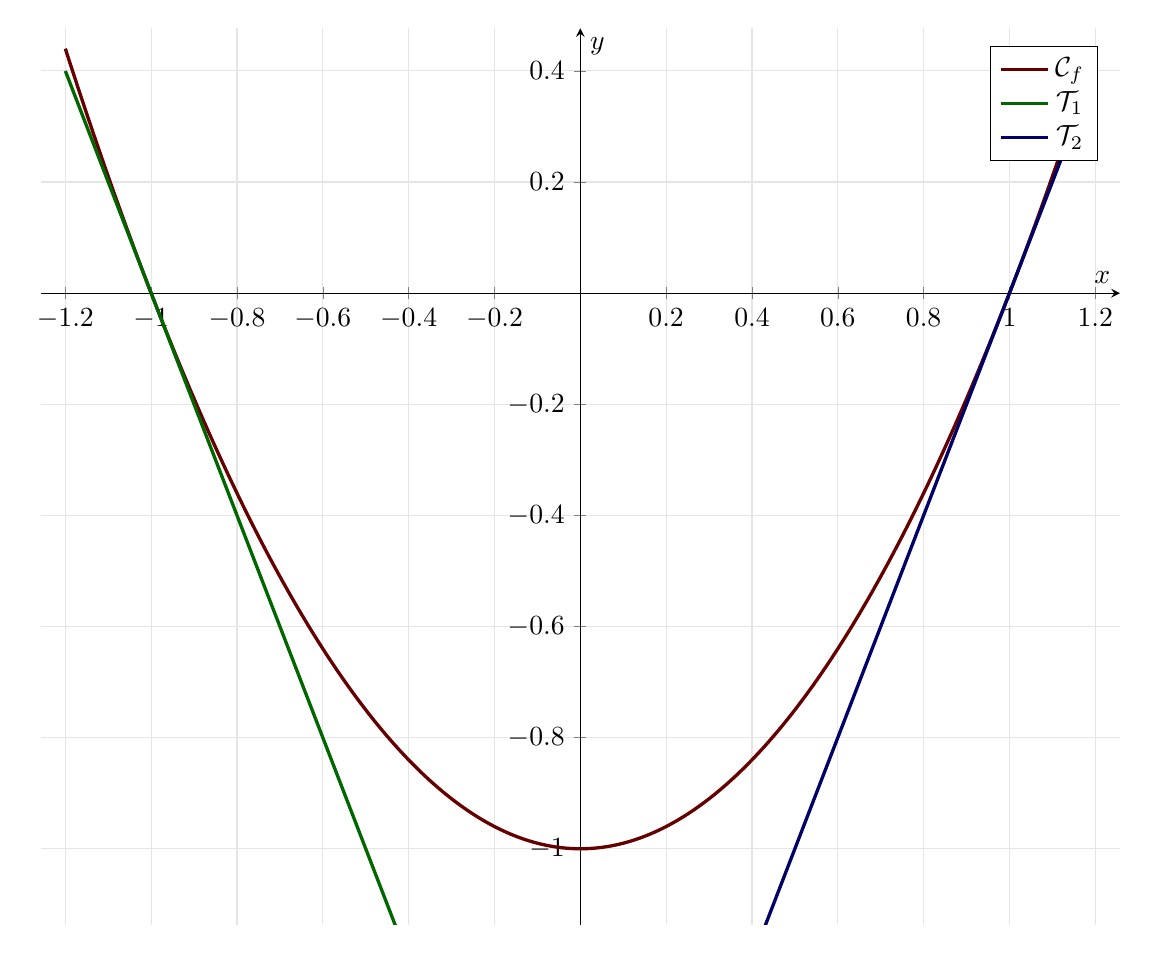
\begin{tikzpicture}[
                declare function={
                    X(\x) = \x;
                    Y(\x) = ((\x)^2) - 1;
                    T(\x) = -2*(\x) - 2;
                    TT(\x) = 2*(\x) - 2;
            },]
            \def\xmi{-1.2}%xmi et xma : intervalle de définition
            \def\xma{1.2}

            \pgfplotsset{grid style={thin,gray!20!white}}
            \pgfplotsset{minor grid style={dotted,red}}
                           
            \begin{axis}[
                    axis lines = center,
                    xlabel = {$x$},
                    ylabel = {$y$},            
                    enlargelimits=(\xma-\xmi)*0.01,
                    grid=both,  
                    scale = 2,
                    ymin = -1.1
                ]
%First curve
                \addplot [
                    domain=\xmi:\xma, 
                    samples=400, 
                    color=black!60!red,
                    very thick,
                ]
                ({X(\x)},{Y(\x)});
                \addlegendentry{$\mathcal{C}_f$}
%First tangent
                \addplot [
                    domain=\xmi:\xma, 
                    samples=400, 
                    color=black!60!green,
                    very thick,
                ]
                ({X(\x)},{T(\x)});
                \addlegendentry{$\mathcal{T}_1$}
%Second tangent
                \addplot [
                    domain=\xmi:\xma, 
                    samples=400, 
                    color=black!60!blue,
                    very thick,
                ]
                ({X(\x)},{TT(\x)});
                \addlegendentry{$\mathcal{T}_2$}
            \end{axis}
    \end{tikzpicture}
\end{center}

Déterminer les valeurs suivantes:

\begin{multicols}{2} 
 $f(-1) = \ldots$ 
 
 $f(0) = \ldots$ 
 
 $f(1) = \ldots$ 
 
 $f'(-1) = \ldots$ 
 
 $f'(0) = \ldots$ 
 
 $f'(1) = \ldots$  
\end{multicols}



\part{Fonction dérivée}

\section{Du nombre dérivé à la fonction dérivée}

On a vu que lorsqu'une fonction $f$ est dérivable sur un intervalle $I$ on peut associer, pour chaque $x \in I$, le nombre dérivé $f'(x)$. 

\begin{definition}{fonction dérivée}
Si $f$ est une fonction dérivable sur un intervalle $I$, sa dérivée est la fonction telle que pour tout $x \in I, f': x \longmapsto f'(x)$. 
\end{definition}

Cette fonction est souvent nommée $f'(x)$ en mathématiques, $\dfrac{\mathrm{d} f}{\mathrm{d} x}$ en physique.

\section{Détermination de la fonction dérivée d'une fonction}

Nous allons voir dans cette partie les propriétés nécessaires au calcul de la fonction dérivée d'une fonction donnée.

\subsection{Propriétés de la dérivation de fonctions}

\subsubsection{Dérivées de fonctions usuelles}

Voici les dérivées des fonctions les plus courantes:

\begin{table}[h!]
\centering
\begin{tabular}{|c|c|}
\hline
\textbf{fonction $f$} & \textbf{dérivée $f'$} \\ \hline
$k, k \in \mathbb{R}$ & $0$ \\  \hline\hline 
 $x^\alpha$, $\alpha \in \mathbb{R}$ & $\alpha \cdot x^{\alpha-1}$ \\ \hline
 $x$ & $1$ \\ \hline
 $\dfrac{1}{x}$ & $-\dfrac{1}{x^2}$ \\ \hline
 $\sqrt{x}$ & $\dfrac{1}{2\sqrt{x}}$ \\ \hline
 $\dfrac{1}{x^n}$ & $-\dfrac{n}{x^{n+1}}$ \\ \hline\hline
  $e^x$ & $e^x$ \\ \hline
  $\ln x$ & $\dfrac{1}{x} $ \\ \hline\hline
 $\sin x$ & $\cos x$ \\ \hline
 $\cos x$ & $-\sin x$ \\ \hline
 $\tan x$ & $1+\tan\left(x\right)^{2}$ \\ \hline
\end{tabular}
 \caption{Dérivées des fonctions usuelles}
 \label{tab:usuelles}
\end{table}

\subsubsection{Propriétés opératoires}

\paragraph{Opérations de base}

Soient deux fonctions $f$ et $g$, et leurs dérivées respectives $f'$ et $g'$ ainsi que $k \in \mathbb{R}$. 

On a alors:

\begin{enumerate}
 \item $(f+g)' = f'+g'$; \label{regle:somme}
 \item $(kf)' = kf'$;
 \item $(uv)' = u'v + uv'$;\label{derivProd}
 \item $\dfrac{u}{v} = \dfrac{u'v - uv'}{v^2}$;\label{derivFrac}
 \item $\dfrac{1}{u} = -\dfrac{u'}{u^2}$ (n'est qu'un cas particulier du point \ref{derivFrac});
\end{enumerate}

\begin{multicols}{2}
\exemple{$f(x) = (2x+1)(x-2)$}

$f$ est de la forme $uv$ avec:

$u(x) = 2x+1$, donc $u'(x) = 2$

$v(x) = x-2$, donc $v'(x) = 1$

On applique donc la formule \ref{derivProd}:

$f'(x) = 2(x-2) + (2x+1) = 4x-3$

\exemple{$f(x) = \dfrac{x+1}{x-1}$ pour $x \in \mathbb{R} - \{1\}$}

$f$ est de la forme $\dfrac{u}{v}$ avec:

$u(x) = x+1$, donc $u'(x) = 1$

$v(x) = x-1$, donc $v'(x) = 1$

Il reste donc à appliquer la formule \ref{derivFrac}:

$f'(x) = \dfrac{(x-1)-(x+1)}{(x-1)^2} = \dfrac{-2}{(x-1)^2}$ 
\end{multicols}

Quelle est la dérivée $f'$ de la fonction $f:x \longmapsto x^3 + 2x - 3$?

\cadre{5}

Calculer la dérivée de la fonction $g$ telle que $g(x) = \dfrac{1}{x^3+1}$

\cadre{4}

\paragraph{Dérivée d'une fonction composée, cas général}

Soient deux fonctions $f$ et $u$, et leurs dérivées respectives $f'$ et $u'$.

On a alors:

\begin{equation}
 (f \circ u)' = u' f'\circ u
 \label{eq:compo}
\end{equation}

Ce qui peut également s'écrire:

\begin{equation}
 (f(u(x)))' = u'(x) \times f'(u(x))
 \label{eq:compox}
\end{equation}

\exemple{La dérivée de la fonction définie sur $\mathbb{R}^+_*$ par $g:x \longmapsto \ln^3 x$}

On reconnaît la fonction $g$ comme étant la composée de 2 fonctions $f$ et $u$ ($g = f \circ u$) où:

\begin{itemize}
 \item $f(x) = \ln x$ donc $f'(x) = \frac{1}{x}$;
 \item $u(x) = x^3$ donc $u'(x) = 3x^2$.
\end{itemize}

En appliquant la formule (\ref{eq:compo}) ou (\ref{eq:compox}), on obtient
$g'(x) = \frac{1}{x} \times 3 \times \ln^2 x$ soit:

\begin{equation*}
 g'(x) = (f \circ u)'(x) = \frac{3}{x} \times \ln^2 x
\end{equation*}

\exemple{La dérivée de la fonction définie sur $\mathbb{R}^+_*$ par $h:x \longmapsto \ln (x^3)$}

On reconnaît la fonction $h$ comme étant la composée de 2 fonctions $u$ et $f$ ($h = u \circ f$) où $f$ et $u$ sont les fonctions de l'exemple précédent.

En appliquant la formule (\ref{eq:compo}) ou (\ref{eq:compox}), on obtient
$h'(x) = \frac{3x^2}{x^3} $ soit (sachant que $x \neq 0$):

\begin{equation*}
 h'(x) = (u \circ f)'(x) = \frac{3}{x}
\end{equation*}

On peut ainsi récapituler le cas général et quelques cas particuliers qui en découlent (table \ref{tab:composees}).

\begin{table}[h!]
\centering
\begin{tabular}{|c|c|}
\hline
 \textbf{Fontion composée} & \textbf{Dérivée} \\ \hline\hline
$u \circ v$  & $v' \times u' \circ v$ \\ \hline\hline
$e^{u}$ & $u' \times e^{u}$ \\ \hline
 $\ln u$ avec $u(x) > 0$ & $\frac{u'}{u} $ \\ \hline
 $\frac{1}{u}$ & $-\frac{u'}{u^2}$ \\ \hline
 $u^n$ & $n u' u^{n-1}$ \\ \hline
 $\sqrt{u}$ & $\frac{u'}{2\sqrt{u}}$ \\ \hline
\end{tabular}
 \caption{Dérivées de composées de fonctions}
 \label{tab:composees}
\end{table}

\textbf{Exemples :}

\begin{enumerate}
 \item Calculer la dérivée de la fonction $x \longmapsto e^{x^2 + 2x + 1}$

\cadre{4}

 \item Soit la fonction $f$ telle que $f(x) = \sqrt{x^2 + x + 1}$. Donner l'expression de $f'$.
 
 \cadre{4}

 \item Déterminer la dérivée de la fonction $\ln (3x+4)$.
 
 \cadre{4}

 \item Déterminer la dérivée de la fonction $x \longmapsto (\ln x + x)^3$.
 
 \cadre{3}
\end{enumerate}

% \section{Applications de la dérivée}

\section{Application: le sens de variation d'une fonction}

\subsection{Introduction}

Soit $f$ une fonction et $f'$ sa dérivée. Connaître le signe de $f'$ nous permet de retrouver les variations de la fonction $f$. 

Plus précisément:

\begin{itemize}
 \item lorsque $f'$ est positive, $f$ est croissante
 \item lorsque $f'$ est négative, $f$ est décroissante
\end{itemize}

Ou encore, avec des inégalités strictes:

\begin{itemize}
 \item lorsque $f'$ est strictement positive, $f$ est strictement croissante
 \item lorsque $f'$ est strictement négative, $f$ est strictement décroissante
\end{itemize}

Ce lien entre la monotonie\footnote{C'est-à-dire le fait qu'elle soit croissante ou décroissante.} de la fonction et le signe de la dérivée est illustré \cref{fig:IllustrationVariation}. 

\begin{figure}[h]
\begin{center}
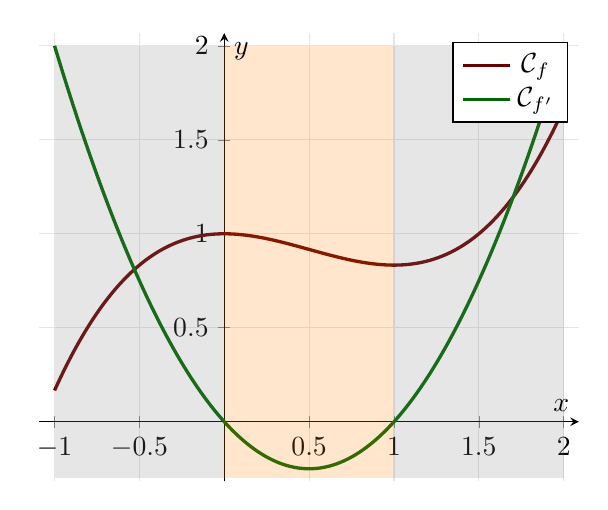
\begin{tikzpicture}[
                declare function={
                    X(\x) = \x;
                    Y(\x) = ((\x)^3)/3 - ((\x)^2)/2 + 1;
                    Z(\x) = ((\x)^2) - (\x);
            },]
            \def\xmi{-1}%xmi et xma : intervalle de définition
            \def\xma{2}

            \pgfplotsset{grid style={thin,gray!20!white}}
            \pgfplotsset{minor grid style={dotted,red}}
                           
            \begin{axis}[
                    axis lines = center,
                    xlabel = {$x$},
                    ylabel = {$y$},            
                    enlargelimits=(\xma-\xmi)*0.01,
                    grid=both,  
                    scale = 1
                ]
%First curve
                \addplot [
                    domain=\xmi:\xma, 
                    samples=400, 
                    color=black!60!red,
                    very thick,
                ]
                ({X(\x)},{Y(\x)});
                \addlegendentry{$\mathcal{C}_f$}
%Second curve
                \addplot [
                    domain=\xmi:\xma, 
                    samples=400, 
                    color=black!60!green,
                    very thick,
                ]
                ({X(\x)},{Z(\x)});
                \addlegendentry{$\mathcal{C}_{f'}$}
                
                \fill [gray,    opacity=0.2] (\xmi,-0.3) rectangle (0,2);
                \fill [orange, opacity=0.2] (0,-0.3) rectangle (1,2);
                \fill [gray,    opacity=0.2] (1,-0.3) rectangle (\xma,2);
            \end{axis}
    \end{tikzpicture}
\end{center}
    \caption{
     En gris (intervalles $[-1;0]$ et $[1;2]$): $f'(x) > 0$ donc $f(x)$ croissante; en orange (intervalle $[0;1]$): $f'(x) < 0$ donc $f(x)$ décroissante.}
    \label{fig:IllustrationVariation}
\end{figure}

Cette propriété est centrale dans l'étude de fonctions.

\subsection{Étude des variations d'une fonction}

Étudier les variations d'une fonction $f$ revient à indiquer: 

\begin{itemize}
 \item les intervalles sur lesquels la fonction $f$ est \textbf{croissante} d'une part;
 \item les intervalles sur lesquels celle-ci $f$ est \textbf{décroissante} d'autre part. 
\end{itemize}

Ceci est équivalent à trouver: 

\begin{itemize}
 \item les intervalles sur lesquels la fonction $f'$ est \textbf{positive} d'une part;
 \item les intervalles sur lesquels celle-ci $f'$ est \textbf{négative} d'autre part. 
\end{itemize}

Le résultat d'une telle étude est souvent donné dans un \emph{tableau de variations}. 

\exemple{}
Soit la fonction $f : x \longmapsto x^2 + 4x + 1$.

On calcule sa dérivée $f'$:

\begin{itemize}
 \item $(x^2)' = 2x$
 \item $(4x)' = 4$
 \item 1 est une constante, sa dérivée est donc 0.
\end{itemize}

Finalement, comme la dérivée d'une somme est la somme des dérivées (règle \ref{regle:somme} page \pageref{regle:somme}), $f'(x) = 2x + 4$. 

On étudie maintenant le signe de $f'(x)$. On peut par exemple résoudre l'équation:

\begin{equation*}
 f'(x) \geqslant 0
\end{equation*}

$$\Leftrightarrow 2x + 4 \geqslant 0$$

$$\Leftrightarrow x \geqslant -2$$

On a donc: 

\begin{itemize}
 \item $f'(x) \geqslant 0 \Leftrightarrow x  \geqslant -2$;
 \item $f'(x) < 0 \Leftrightarrow x  < -2$.
\end{itemize}

soit:

\begin{itemize}
 \item $f(x)$ croissante sur $[-2 ; +\infty[$;
 \item $f(x)$ décroissante sur $]-\infty ; -2]$;
\end{itemize}

Ce résultat peut être synthétisé dans le tableau de signe de $f'$, dont on déduira le tableau de variation de $f$. 

Dans la pratique, on superpose souvent les deux dans un seul tableau (table \ref{tab:VarExemple}).

\begin{table}[h]
\begin{center}
\begin{tikzpicture}
   \tkzTabInit{$x$ / 1 , $f'(x)$ / 1 , $f(x)$ / 2}{$-\infty$, $-2$, $+\infty$}
   \tkzTabLine{, -, z, +, }
   \tkzTabVar{+/ $+\infty$, -/ $-3$, +/ $+\infty$}
\end{tikzpicture} 
\end{center}
\caption{Tableau de variation de la fonction $f$}
\label{tab:VarExemple}
\end{table}

\exemple{}
Étudier les variations de la fonction $g$ telle que $g(x) = \dfrac{1}{2}x^{2} + 3x + 1$.

\cadre{8}

\exemple{}
Étudier les variations de la fonction $h : x \longmapsto \dfrac{1}{3}x^{3}+\dfrac{1}{2}x^{2}-2 x$.

\cadre{10}

\section*{Exercices}

\exo{}


\end{document}

